% =============================================================================
% APPENDIX BX: CORE-BEATRIX: Technical Architecture of LLM-Framework Symbiosis
% =============================================================================
% Module: BCM2_00_META
% Version: 1.1 (January 2026)
% Status: Draft
%
% v1.1 Updates:
% - Added three-tier hierarchy (LLM → Agent → BEATRIX)
% - Added technically precise terminology table (non-anthropomorphic language)
% - Added Figure bx-hierarchy and Table bx-tiers
%
% This appendix provides a deep technical explanation of what happens
% inside a pure LLM vs. EBF/BEATRIX - layer by layer, component by component.
%
% =============================================================================

% =============================================================================
% CROSS-REFERENCE STRUCTURE
% =============================================================================
%
% CHAPTER LINKAGE (Required):
% - Primary Chapter: Chapter 1 (Introduction to EBF)
% - Secondary Chapters: Chapter 4 (Empirical Foundations), Chapter 17 (Interventions)
%
% DEPENDENCIES (what this appendix REQUIRES):
% - Appendix UNMAPPED_FM: METHOD-FRAMEWORK (Framework principles)
% - Appendix G: Glossary
%
% DEPENDENTS (what REQUIRES this appendix):
% - All future BEATRIX documentation
% - Innosuisse proposal technical sections
%
% =============================================================================

\begin{tcolorbox}[colback=purple!5!white, colframe=purple!75!black,
    title=Chapter Linkage]

\textbf{Primary Chapter:} Chapter 1: Introduction to EBF
\begin{itemize}[nosep]
\item Section 1.1: What is EBF? $\leftrightarrow$ This Appendix Section \ref{sec:bx-architecture}
\item Section 1.5: EBF Technology $\leftrightarrow$ This Appendix Section \ref{sec:bx-comparison}
\end{itemize}

\textbf{Secondary Chapters:}
\begin{itemize}[nosep]
\item Chapter 4: Empirical Foundations --- references parameter validation
\item Chapter 17: Interventions --- uses model registry
\end{itemize}

\textbf{Reading Guide:}
\begin{itemize}[nosep]
\item For business perspective: Read Appendix UNMAPPED_FM first
\item For technical deep-dive: This appendix provides complete specification
\item For implementation: See BEATRIX technical documentation
\end{itemize}

\end{tcolorbox}

\chapter{CORE-BEATRIX: Technical Architecture of LLM-Framework Symbiosis}
\label{app:core-beatrix}


\begin{tcolorbox}[colback=blue!5!white, colframe=blue!75!black,
    title=Quick Reference: Appendix UNMAPPED_BX]

\textbf{Appendix:} BX (CORE-BEATRIX)

\textbf{Core Question:} What happens technically inside a pure LLM vs. BEATRIX, and why does this create fundamentally different scalability properties?

\textbf{Key Formula:}
\begin{equation}
\text{BEATRIX} = \underbrace{\text{LLM}}_{\text{Generation}} \times \underbrace{\mathcal{S}}_{\text{Structure}} \times \underbrace{\mathcal{D}}_{\text{Data}} \times \underbrace{\mathcal{V}}_{\text{Validation}}
\label{eq:bx-core}
\end{equation}

\textbf{Key Concepts:}
\begin{itemize}[nosep]
\item \textbf{Three-Tier Hierarchy}: Pure LLM → LLM-Agent → BEATRIX
\item \textbf{Technically Precise Language}: LLMs don't ``think''---they execute Forward Passes
\item \textbf{Context Window vs. Persistent Memory}: LLM forgets; BEATRIX accumulates
\item \textbf{Implicit vs. Explicit Parameters}: LLM weights are fixed; BEATRIX parameters update
\end{itemize}

\textbf{Cross-References:} Appendix UNMAPPED_FM (Framework), BBB (Parameters), FFF (Registry), G (Glossary)
\end{tcolorbox}


\begin{abstract}
This appendix provides a technically rigorous explanation of the architectural differences between a pure Large Language Model (LLM) and BEATRIX (EBF + LLM). We introduce a \textbf{three-tier hierarchy}---Pure LLM → LLM-Agent → BEATRIX---and analyze what happens at each processing layer using \textbf{technically precise, non-anthropomorphic language} (LLMs execute Forward Passes, not ``thinking''). We identify seven fundamental asymmetries that create different scalability properties. The core insight: LLMs are \textit{stateless pattern matchers}; LLM-Agents add tool use but remain stateless; BEATRIX adds structure, data, validation, and persistence to become a \textit{stateful knowledge system}. This distinction explains why consulting insights disappear while BEATRIX knowledge accumulates.
\end{abstract}


\begin{tcolorbox}[
    colback=orange!5!white,
    colframe=orange!75!black,
    title={\textbf{Appendix Scope: Ziel / In-Scope / Out-of-Scope / Constraints}},
    fonttitle=\bfseries
]

\textbf{Ziel (Objective):}
\begin{itemize}[nosep]
    \item Provide a complete technical specification of what happens inside a pure LLM vs. BEATRIX, explaining why BEATRIX scales and pure LLMs do not
\end{itemize}

\textbf{In-Scope:}
\begin{itemize}[nosep]
    \item \textbf{Three-tier hierarchy}: Pure LLM → LLM-Agent → BEATRIX
    \item \textbf{Technically precise terminology}: Non-anthropomorphic language for LLM operations
    \item Technical architecture of LLMs (tokenization, attention, generation)
    \item Technical architecture of BEATRIX (constraints, registries, validation)
    \item Layer-by-layer comparison
    \item Seven scalability axioms (UNMAPPED_BX-1 to UNMAPPED_BX-7)
    \item Mathematical proof of scalability difference
\end{itemize}

\textbf{Out-of-Scope (delegiert an andere Appendices):}
\begin{itemize}[nosep]
    \item Business implications of scalability $\rightarrow$ Appendix UNMAPPED_FM (METHOD-FRAMEWORK)
    \item Specific parameter values $\rightarrow$ Appendix UNMAPPED_BBB (CORE-WHERE)
    \item Model design workflows $\rightarrow$ Appendix EEE (METHOD-DESIGN)
\end{itemize}

\textbf{Constraints (Anwendungsgrenzen):}
\begin{itemize}[nosep]
    \item Technical details may change as LLM technology evolves
    \item Implementation details are BEATRIX-specific
    \item Assumes familiarity with basic ML/AI concepts
\end{itemize}

\textbf{Lieferobjekte (Deliverables):}
\begin{itemize}[nosep]
    \item Three-tier hierarchy diagram (Figure \ref{fig:bx-hierarchy})
    \item Technically precise terminology table (non-anthropomorphic language)
    \item Complete processing pipeline comparison (Table \ref{tab:bx-pipeline})
    \item Seven scalability axioms (UNMAPPED_BX-1 to UNMAPPED_BX-7)
    \item Formal scalability proof (Theorem \ref{thm:bx-scalability})
    \item Three-tier comparison table (Table \ref{tab:bx-tiers})
\end{itemize}

\end{tcolorbox}


%%%%%%%%%%%%%%%%%%%%%%%%%%%%%%%%%%%%%%%%%%%%%%%%%%%%%%%%%%%%%%%%%%%%%%%%%%%%%%%
% NAMING CONVENTION
%%%%%%%%%%%%%%%%%%%%%%%%%%%%%%%%%%%%%%%%%%%%%%%%%%%%%%%%%%%%%%%%%%%%%%%%%%%%%%%

\begin{tcolorbox}[colback=blue!10!white, colframe=blue!75!black,
    title=\textbf{Naming Convention: BEATRIX = EBF}]

\textbf{BEATRIX} is the FehrAdvice \& Partners AG brand name for EBF when deployed as a product or service.

\begin{table}[H]
\centering
\renewcommand{\arraystretch}{1.3}
\begin{tabular}{@{}lp{9cm}@{}}
\toprule
\textbf{Term} & \textbf{Meaning} \\
\midrule
\textbf{EBF} & \textbf{Evidence-Based Framework of Economic and Social Behavior} (full scientific name) \\
\textbf{BEATRIX} & EBF branded for FehrAdvice \& Partners AG (product name) \\
\textbf{10C Framework} & The structural core of EBF (10 CORE questions) \\
\textbf{LLM} & Large Language Model (e.g., Claude, GPT) \\
\bottomrule
\end{tabular}
\end{table}

\textbf{In this appendix:} ``BEATRIX'' and ``EBF'' are used interchangeably. The technical architecture is identical; only the branding differs.

\end{tcolorbox}


%%%%%%%%%%%%%%%%%%%%%%%%%%%%%%%%%%%%%%%%%%%%%%%%%%%%%%%%%%%%%%%%%%%%%%%%%%%%%%%
% TECHNICALLY PRECISE TERMINOLOGY
%%%%%%%%%%%%%%%%%%%%%%%%%%%%%%%%%%%%%%%%%%%%%%%%%%%%%%%%%%%%%%%%%%%%%%%%%%%%%%%

\begin{tcolorbox}[colback=yellow!10!white, colframe=yellow!75!black,
    title=\textbf{Technically Precise Terminology: LLMs Do Not ``Think''}]

To avoid anthropomorphic misconceptions, this appendix uses \textbf{technically precise language} for LLM operations. The following table maps colloquial terms to their actual computational processes:

\begin{table}[H]
\centering
\renewcommand{\arraystretch}{1.4}
\begin{tabular}{@{}p{2.5cm}p{4cm}p{5.5cm}@{}}
\toprule
\textbf{Colloquial} & \textbf{Technical Term} & \textbf{What Actually Happens} \\
\midrule
``thinks'' & Forward Pass & Attention mechanism + Feed-Forward Network layers \\
``understands'' & Pattern Matching & Similarity computation in embedding space \\
``decides'' & Token Sampling & Probabilistic selection from softmax distribution \\
``remembers'' & Context Window Retrieval & Attention over tokens currently in context \\
``learns'' & Weight Update & Gradient descent during training (not inference) \\
``knows'' & Weight Encoding & Information implicit in model parameters \\
``reasons'' & Chain of Tokens & Sequential token generation with self-attention \\
``creates'' & Stochastic Generation & Temperature-controlled sampling from distribution \\
\bottomrule
\end{tabular}
\end{table}

\textbf{Why this matters:} Anthropomorphic language creates false expectations. Users expect LLMs to ``remember'' previous conversations (they don't---context window is cleared). Users expect LLMs to ``learn'' from corrections (they don't---weights are frozen at inference).

\end{tcolorbox}


%%%%%%%%%%%%%%%%%%%%%%%%%%%%%%%%%%%%%%%%%%%%%%%%%%%%%%%%%%%%%%%%%%%%%%%%%%%%%%%
% THREE-TIER HIERARCHY
%%%%%%%%%%%%%%%%%%%%%%%%%%%%%%%%%%%%%%%%%%%%%%%%%%%%%%%%%%%%%%%%%%%%%%%%%%%%%%%

\section{The Three-Tier Hierarchy: LLM → Agent → BEATRIX}
\label{sec:bx-hierarchy}

A common confusion conflates three distinct system tiers. Each tier adds capabilities but also complexity:

\begin{figure}[htbp]
\centering
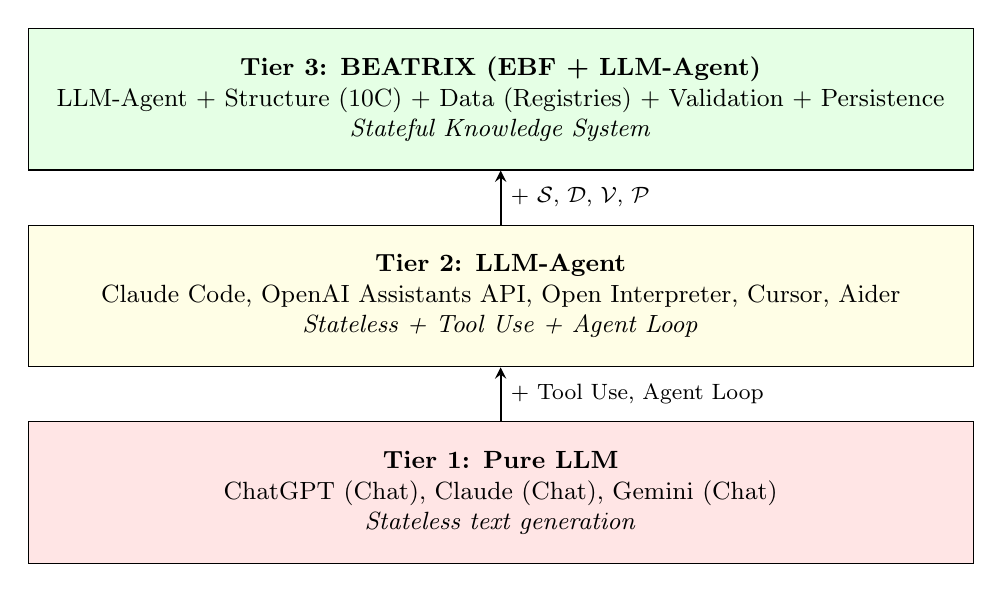
\begin{tikzpicture}[
    tier/.style={rectangle, draw, minimum width=12cm, minimum height=1.8cm, align=center, font=\small},
    arrow/.style={->, thick, >=stealth}
]

% Tier 1
\node[tier, fill=red!10] (t1) at (0,0) {
    \textbf{Tier 1: Pure LLM} \\
    ChatGPT (Chat), Claude (Chat), Gemini (Chat) \\
    \textit{Stateless text generation}
};

% Tier 2
\node[tier, fill=yellow!10] (t2) at (0,2.5) {
    \textbf{Tier 2: LLM-Agent} \\
    Claude Code, OpenAI Assistants API, Open Interpreter, Cursor, Aider \\
    \textit{Stateless + Tool Use + Agent Loop}
};

% Tier 3
\node[tier, fill=green!10] (t3) at (0,5) {
    \textbf{Tier 3: BEATRIX (EBF + LLM-Agent)} \\
    LLM-Agent + Structure (10C) + Data (Registries) + Validation + Persistence \\
    \textit{Stateful Knowledge System}
};

% Arrows
\draw[arrow] (t1.north) -- (t2.south) node[midway, right, font=\footnotesize] {+ Tool Use, Agent Loop};
\draw[arrow] (t2.north) -- (t3.south) node[midway, right, font=\footnotesize] {+ $\mathcal{S}$, $\mathcal{D}$, $\mathcal{V}$, $\mathcal{P}$};

\end{tikzpicture}
\caption{Three-Tier Hierarchy: From Pure LLM to BEATRIX}
\label{fig:bx-hierarchy}
\end{figure}

\subsection{Tier 1: Pure LLM (Chat Interfaces)}

\textbf{Examples:} ChatGPT (browser), Claude.ai (browser), Gemini (browser)

\textbf{Architecture:}
\begin{equation}
\text{Tier 1} = \text{Forward Pass}(\text{Prompt}) \rightarrow \text{Token Sampling} \rightarrow \text{Response}
\end{equation}

\textbf{Characteristics:}
\begin{itemize}[nosep]
    \item Input: User text prompt
    \item Processing: Single forward pass through transformer layers
    \item Output: Generated text
    \item State: None (context window cleared between sessions)
    \item Tools: None
\end{itemize}

\textbf{Technical Process:}
\begin{enumerate}
    \item \textbf{Tokenization:} Input string → token IDs
    \item \textbf{Embedding Lookup:} Token IDs → vectors in $\mathbb{R}^d$
    \item \textbf{Self-Attention:} $\text{softmax}(QK^T/\sqrt{d_k})V$ across all layers
    \item \textbf{Feed-Forward:} Non-linear transformation per position
    \item \textbf{Output Projection:} Hidden state → vocabulary logits
    \item \textbf{Sampling:} Probabilistic token selection (temperature, top-k, top-p)
    \item \textbf{Repeat:} Until end-of-sequence token or max length
\end{enumerate}


\subsection{Tier 2: LLM-Agent (Tool-Using Systems)}

\textbf{Examples:} Claude Code (CLI), OpenAI Assistants API, Open Interpreter, Cursor, Aider, GitHub Copilot

\textbf{Architecture:}
\begin{equation}
\text{Tier 2} = \text{While}(\neg\text{done}) \left\{ \text{Forward Pass} \rightarrow \text{Tool Call?} \rightarrow \text{Execute} \rightarrow \text{Append Context} \right\}
\end{equation}

\textbf{What Tier 2 adds:}
\begin{itemize}[nosep]
    \item \textbf{Agent Loop:} Model can call tools and receive results
    \item \textbf{Tool Use:} File read/write, shell commands, web requests, code execution
    \item \textbf{Context Accumulation:} Tool results appended to context within session
    \item \textbf{Multi-Turn Planning:} Model can break tasks into steps
\end{itemize}

\textbf{Technical Process (Agent Loop):}
\begin{enumerate}
    \item \textbf{Forward Pass:} Generate next tokens
    \item \textbf{Tool Detection:} Check if output is a tool call
    \item \textbf{If Tool Call:}
    \begin{enumerate}
        \item Parse tool name and arguments
        \item Execute tool (e.g., read file, run command)
        \item Append tool result to context
        \item Return to step 1
    \end{enumerate}
    \item \textbf{If Text:} Return response to user
    \item \textbf{Session End:} Context window cleared (no persistence)
\end{enumerate}

\textbf{Critical Limitation:} Tier 2 agents are still \textbf{stateless between sessions}. Claude Code can read files and execute commands \textit{during} a session, but retains nothing \textit{after} the session ends.

\begin{tcolorbox}[colback=red!5!white, colframe=red!75!black,
    title=Why Tier 2 Is Not Enough]
A Tier 2 agent (e.g., Claude Code without EBF) can:
\begin{itemize}[nosep]
    \item Read a file and answer questions about it
    \item Execute code and interpret results
    \item Make multiple tool calls in sequence
\end{itemize}

A Tier 2 agent \textbf{cannot}:
\begin{itemize}[nosep]
    \item Accumulate knowledge across sessions
    \item Guarantee consistent methodology (no enforced structure)
    \item Validate predictions against outcomes
    \item Improve with usage (no learning loop)
\end{itemize}

\textbf{Result:} Query 1000 is identical to query 1. No scalability.
\end{tcolorbox}


\subsection{Tier 3: BEATRIX (Knowledge System)}

\textbf{Definition:} BEATRIX = Tier 2 Agent + $\mathcal{S}$ (Structure) + $\mathcal{D}$ (Data) + $\mathcal{V}$ (Validation) + $\mathcal{P}$ (Persistence)

\textbf{Architecture:}
\begin{equation}
\text{Tier 3} = \text{Agent Loop} \times \underbrace{\text{10C Constraints}}_{\mathcal{S}} \times \underbrace{\text{Registries}}_{\mathcal{D}} \times \underbrace{\text{Falsifiable Outputs}}_{\mathcal{V}} \times \underbrace{\text{Learning Loop}}_{\mathcal{P}}
\end{equation}

\textbf{What Tier 3 adds:}

\begin{table}[htbp]
\centering
\caption{Tier 3 Additions to Tier 2}
\renewcommand{\arraystretch}{1.3}
\begin{tabular}{@{}llp{7cm}@{}}
\toprule
\textbf{Component} & \textbf{Symbol} & \textbf{Implementation} \\
\midrule
Structure & $\mathcal{S}$ & CLAUDE.md injects 10C workflow constraints \\
Data & $\mathcal{D}$ & 6 registries (models, cases, parameters, theories, sessions, outputs) \\
Validation & $\mathcal{V}$ & Monte Carlo predictions with confidence intervals \\
Persistence & $\mathcal{P}$ & Git commits, YAML updates, session logs \\
\bottomrule
\end{tabular}
\end{table}

\textbf{The Critical Insight:}
\begin{equation}
\boxed{\text{Tier 3} = \text{Tier 2} + \text{What the LLM cannot provide}}
\end{equation}

The LLM (Tier 1) provides generation capability. The Agent (Tier 2) provides tool use. The Framework (Tier 3) provides structure, knowledge, validation, and learning---none of which emerge from the LLM itself.


\subsection{Comparison Table: Three Tiers}

\begin{table}[htbp]
\centering
\caption{Three-Tier Comparison: Capabilities and Limitations}
\label{tab:bx-tiers}
\renewcommand{\arraystretch}{1.4}
\begin{tabular}{@{}p{3cm}ccc@{}}
\toprule
\textbf{Capability} & \textbf{Tier 1} & \textbf{Tier 2} & \textbf{Tier 3} \\
 & Pure LLM & LLM-Agent & BEATRIX \\
\midrule
Text generation & \checkmark & \checkmark & \checkmark \\
Tool use & $\times$ & \checkmark & \checkmark \\
File access & $\times$ & \checkmark & \checkmark \\
Code execution & $\times$ & \checkmark & \checkmark \\
Multi-turn planning & $\times$ & \checkmark & \checkmark \\
\midrule
Enforced structure & $\times$ & $\times$ & \checkmark \\
External knowledge & $\times$ & $\times$ & \checkmark \\
Falsifiable predictions & $\times$ & $\times$ & \checkmark \\
Cross-session persistence & $\times$ & $\times$ & \checkmark \\
Cumulative learning & $\times$ & $\times$ & \checkmark \\
\midrule
\textbf{Scalability} & \textbf{None} & \textbf{None} & \textbf{$O(N \log N)$} \\
\bottomrule
\end{tabular}
\end{table}


%%%%%%%%%%%%%%%%%%%%%%%%%%%%%%%%%%%%%%%%%%%%%%%%%%%%%%%%%%%%%%%%%%%%%%%%%%%%%%%
\section{The Fundamental Question}
\label{sec:bx-fundamental}
%%%%%%%%%%%%%%%%%%%%%%%%%%%%%%%%%%%%%%%%%%%%%%%%%%%%%%%%%%%%%%%%%%%%%%%%%%%%%%%

\subsection{Why This Matters}

Consider two systems answering the same question 1,000 times:

\begin{table}[htbp]
\centering
\caption{Same Question, 1000 Times: LLM vs. BEATRIX}
\label{tab:bx-1000}
\renewcommand{\arraystretch}{1.4}
\begin{tabular}{@{}lcc@{}}
\toprule
\textbf{Property} & \textbf{Pure LLM} & \textbf{BEATRIX} \\
\midrule
Answer consistency & Variable & Deterministic structure \\
Quality at query 1 & $Q_0$ & $Q_0$ \\
Quality at query 1000 & $Q_0$ (unchanged) & $Q_0 + \Delta Q$ (improved) \\
Knowledge retained & 0 & 999 cases + parameters \\
Marginal cost query 1000 & = query 1 & $<$ query 1 \\
\bottomrule
\end{tabular}
\end{table}

The pure LLM treats each query as independent. BEATRIX treats each query as an opportunity to learn. This is not a feature difference---it is an \textbf{architectural asymmetry}.

\subsection{The Core Problem}

\begin{tcolorbox}[colback=red!5!white, colframe=red!75!black,
    title=The Fundamental Question]
\textbf{What happens technically---layer by layer, component by component---inside a pure LLM vs. BEATRIX, and how does this create fundamentally different scalability properties?}
\end{tcolorbox}


%%%%%%%%%%%%%%%%%%%%%%%%%%%%%%%%%%%%%%%%%%%%%%%%%%%%%%%%%%%%%%%%%%%%%%%%%%%%%%%
\section{Technical Architecture: Pure LLM}
\label{sec:bx-llm}
%%%%%%%%%%%%%%%%%%%%%%%%%%%%%%%%%%%%%%%%%%%%%%%%%%%%%%%%%%%%%%%%%%%%%%%%%%%%%%%

\subsection{The LLM Processing Pipeline}

A Large Language Model processes input through the following stages:

\begin{equation}
\text{Input} \xrightarrow{\text{Tokenize}} \text{Tokens} \xrightarrow{\text{Embed}} \text{Vectors} \xrightarrow{\text{Attend}} \text{Context} \xrightarrow{\text{Generate}} \text{Output}
\end{equation}

\subsubsection{Layer 1: Tokenization}

The input text is split into tokens (subword units):

\begin{verbatim}
Input: "How many customers will upgrade?"
Tokens: ["How", " many", " customers", " will", " upgrade", "?"]
Token IDs: [2437, 1784, 6444, 481, 16062, 30]
\end{verbatim}

\textbf{Technical detail:} Tokenization is deterministic. The same input always produces the same tokens. This is \textit{not} where variability enters.

\subsubsection{Layer 2: Embedding}

Each token ID maps to a learned vector in $\mathbb{R}^d$ (typically $d = 4096$ for large models):

\begin{equation}
\mathbf{e}_i = \mathbf{E}[\text{token}_i] \in \mathbb{R}^d
\end{equation}

where $\mathbf{E} \in \mathbb{R}^{V \times d}$ is the embedding matrix with vocabulary size $V \approx 50,000-100,000$.

\textbf{Technical detail:} Embeddings are \textit{fixed after training}. The model cannot update them based on new information.

\subsubsection{Layer 3: Attention (The Core Mechanism)}

The transformer computes attention over the context window:

\begin{equation}
\text{Attention}(Q, K, V) = \text{softmax}\left(\frac{QK^T}{\sqrt{d_k}}\right) V
\end{equation}

where:
\begin{itemize}[nosep]
    \item $Q = XW_Q$ (queries from input)
    \item $K = XW_K$ (keys from context)
    \item $V = XW_V$ (values from context)
    \item $d_k$ = dimension of keys (typically 64-128)
\end{itemize}

\textbf{Critical limitation:} The context window has fixed size $C$ (typically 8K-200K tokens). Information beyond this window is \textit{invisible} to the model.

\begin{tcolorbox}[colback=yellow!5!white, colframe=yellow!75!black,
    title=Technical Insight: The Context Window Problem]
An LLM with context window $C = 100,000$ tokens can ``see'' approximately 75,000 words---roughly one book.

A knowledge system like BEATRIX has access to:
\begin{itemize}[nosep]
    \item 2,328 papers (bibliography)
    \item 852 cases (case registry)
    \item 153 theories (theory catalog)
    \item 400+ parameters (parameter database)
\end{itemize}

This is $\approx 10^7$ tokens of structured knowledge---100$\times$ more than any context window.
\end{tcolorbox}

\subsubsection{Layer 4: Generation (Next Token Prediction)}

The model predicts the next token probabilistically:

\begin{equation}
P(\text{token}_{t+1} | \text{token}_{1:t}) = \text{softmax}(\mathbf{W}_{\text{out}} \cdot \mathbf{h}_t)
\end{equation}

where $\mathbf{h}_t$ is the hidden state after processing tokens $1$ through $t$.

\textbf{Critical insight:} Generation is \textit{stochastic}. The same input can produce different outputs due to:
\begin{enumerate}
    \item Temperature sampling: $P'_i = P_i^{1/T} / \sum_j P_j^{1/T}$
    \item Top-k/Top-p filtering
    \item Random seed variation
\end{enumerate}

\subsubsection{Layer 5: Session Termination}

When the session ends:

\begin{equation}
\text{State}_{\text{after}} = \emptyset
\end{equation}

\textbf{The LLM retains nothing.} No parameters update. No cases are stored. No learning occurs.


\subsection{What the LLM ``Knows''}

The knowledge in an LLM is encoded in its weights $\mathbf{W}$:

\begin{equation}
\text{Knowledge}_{\text{LLM}} = f(\mathbf{W}) \quad \text{where} \quad \mathbf{W} \in \mathbb{R}^{N}, \quad N \approx 10^{11}
\end{equation}

\textbf{Properties of weight-encoded knowledge:}
\begin{enumerate}
    \item \textbf{Implicit:} Cannot be inspected or verified directly
    \item \textbf{Static:} Fixed after training (no updates from user interactions)
    \item \textbf{Entangled:} Individual facts cannot be extracted or corrected
    \item \textbf{Probabilistic:} Retrieved via sampling, not lookup
\end{enumerate}

\begin{tcolorbox}[colback=red!5!white, colframe=red!75!black,
    title=The Hallucination Problem]
Because knowledge is implicit and probabilistic, the LLM cannot distinguish between:
\begin{itemize}[nosep]
    \item Facts learned from training data
    \item Plausible-sounding patterns
    \item Complete fabrications
\end{itemize}

There is no internal ``confidence score'' for factual accuracy. The model generates text that \textit{looks right}, not text that \textit{is right}.
\end{tcolorbox}


%%%%%%%%%%%%%%%%%%%%%%%%%%%%%%%%%%%%%%%%%%%%%%%%%%%%%%%%%%%%%%%%%%%%%%%%%%%%%%%
\section{Technical Architecture: BEATRIX (EBF + LLM)}
\label{sec:bx-architecture}
%%%%%%%%%%%%%%%%%%%%%%%%%%%%%%%%%%%%%%%%%%%%%%%%%%%%%%%%%%%%%%%%%%%%%%%%%%%%%%%

BEATRIX adds four architectural layers to the base LLM:

\begin{equation}
\text{BEATRIX} = \text{LLM} + \underbrace{\mathcal{S}}_{\text{Structure}} + \underbrace{\mathcal{D}}_{\text{Data}} + \underbrace{\mathcal{V}}_{\text{Validation}} + \underbrace{\mathcal{P}}_{\text{Persistence}}
\end{equation}

\subsection{Layer S: Structural Constraints (10C Framework)}

The 10C Framework constrains the LLM's output space:

\begin{equation}
\text{Output}_{\text{BEATRIX}} \in \mathcal{O}_{10C} \subset \mathcal{O}_{\text{LLM}}
\end{equation}

where $\mathcal{O}_{10C}$ is the set of outputs that satisfy 10C structural requirements.

\textbf{Implementation:} The CLAUDE.md file injects structural constraints into every prompt:

\begin{verbatim}
PFLICHT: Bei JEDER inhaltlichen Frage
  SCHRITT 0: Session starten
  SCHRITT 1: Kontext verstehen (Ψ-Dimensionen)
  SCHRITT 2: Modell auswählen (aus Registry)
  SCHRITT 3: Parameter bestimmen (aus BBB)
  SCHRITT 4: Analyse & Antwort
  ...
\end{verbatim}

\textbf{Technical effect:} The LLM's generation is constrained to follow a deterministic workflow. Variability in \textit{structure} is eliminated; variability in \textit{parameters} remains but is bounded by empirical data.

\begin{tcolorbox}[colback=gray!5!white, colframe=gray!75!black,
    title=Axiom UNMAPPED_BX-1: Structural Constraint]
\textbf{Statement:} Let $\mathcal{S}$ be a structural constraint system. Then:
\begin{equation}
H(\text{Output} | \mathcal{S}) < H(\text{Output})
\end{equation}
where $H(\cdot)$ denotes entropy.

\textbf{Interpretation:} Structural constraints reduce output entropy (variability). The same question produces more consistent answers.

\textbf{Implication:} Reproducibility emerges from structure, not from the LLM itself.
\end{tcolorbox}


\subsection{Layer D: External Data (Registries and Databases)}

BEATRIX connects to persistent data stores:

\begin{table}[htbp]
\centering
\caption{BEATRIX Data Architecture}
\label{tab:bx-data}
\renewcommand{\arraystretch}{1.3}
\begin{tabular}{@{}llll@{}}
\toprule
\textbf{Store} & \textbf{Content} & \textbf{Size} & \textbf{Access} \\
\midrule
\texttt{bcm\_master.bib} & Papers & 2,328 & Citation lookup \\
\texttt{model-registry.yaml} & Models & 13+ & Model selection \\
\texttt{case-registry.yaml} & Cases & 852 & Case matching \\
\texttt{theory-catalog.yaml} & Theories & 153 & Theory grounding \\
\texttt{parameter-registry.yaml} & Parameters & 400+ & Value lookup \\
\texttt{model-building-session.yaml} & Sessions & 14+ & Learning loop \\
\bottomrule
\end{tabular}
\end{table}

\textbf{Technical implementation:}

\begin{verbatim}
# Parameter lookup (not LLM generation)
lambda_CH = parameter_registry["PAR-UNMAPPED_PT-001"]["value"]  # 2.1
sigma_SQ = parameter_registry["PAR-SQ-001"]["value"]   # 0.78

# Model lookup (not LLM generation)
model = model_registry["MOD-ALPM-002"]
formula = model["formula"]  # P(Upgrade) = P(Aware) × Σ[...]
\end{verbatim}

\begin{tcolorbox}[colback=gray!5!white, colframe=gray!75!black,
    title=Axiom UNMAPPED_BX-2: Explicit Knowledge]
\textbf{Statement:} Let $K_{\text{explicit}}$ denote knowledge stored in structured databases. Then:
\begin{equation}
\text{Verifiable}(K_{\text{explicit}}) = 1 \quad \text{vs.} \quad \text{Verifiable}(K_{\text{LLM}}) \approx 0
\end{equation}

\textbf{Interpretation:} Explicit knowledge can be inspected, verified, and corrected. LLM knowledge cannot.

\textbf{Implication:} BEATRIX can guarantee ``$\lambda = 2.1$ comes from Kahneman \& Tversky (1979)''. The LLM cannot.
\end{tcolorbox}


\subsection{Layer V: Validation (Falsifiable Predictions)}

BEATRIX generates predictions with confidence intervals:

\begin{equation}
\hat{y} = 0.67\% \quad \text{with} \quad \text{CI}_{90\%} = [0.25\%, 1.38\%]
\end{equation}

\textbf{Technical implementation:}

\begin{verbatim}
# Monte Carlo simulation (10,000 draws)
draws = []
for i in range(10000):
    lambda_i = np.random.normal(2.1, 0.3)  # Prior uncertainty
    sigma_i = np.random.normal(0.78, 0.05)
    p_i = compute_probability(lambda_i, sigma_i, ...)
    draws.append(p_i)

prediction = np.median(draws)
ci_lower = np.percentile(draws, 5)
ci_upper = np.percentile(draws, 95)
\end{verbatim}

\begin{tcolorbox}[colback=gray!5!white, colframe=gray!75!black,
    title=Axiom UNMAPPED_BX-3: Falsifiability]
\textbf{Statement:} A system is falsifiable if it generates predictions $\hat{y}$ that can be compared to observations $y$:
\begin{equation}
\exists \, y : |y - \hat{y}| > \epsilon \implies \text{Revise model}
\end{equation}

\textbf{Interpretation:} If BEATRIX predicts 0.67\% and Assura observes 2.5\%, the model is wrong and must be revised.

\textbf{Implication:} BEATRIX can learn from being wrong. An LLM generating ``1-3\%'' cannot be falsified.
\end{tcolorbox}


\subsection{Layer P: Persistence (The Learning Loop)}

After each session, BEATRIX updates its knowledge stores:

\begin{verbatim}
# After Assura analysis
session_registry.append({
    "id": "EBF-S-2026-01-29-FIN-001",
    "model": "MOD-ALPM-002",
    "prediction": 0.0067,
    "ci": [0.0025, 0.0138],
    "outcome": null  # To be filled when observed
})

model_registry.update({
    "MOD-ALPM-002": {
        "applications": 1,
        "last_used": "2026-01-29"
    }
})
\end{verbatim}

\begin{tcolorbox}[colback=gray!5!white, colframe=gray!75!black,
    title=Axiom UNMAPPED_BX-4: Cumulative Learning]
\textbf{Statement:} Let $K_t$ denote system knowledge at time $t$. For BEATRIX:
\begin{equation}
K_{t+1} = K_t + \Delta K_t \quad \text{where} \quad \Delta K_t \geq 0
\end{equation}

For a pure LLM:
\begin{equation}
K_{t+1} = K_t \quad \text{(no change)}
\end{equation}

\textbf{Interpretation:} BEATRIX accumulates knowledge monotonically. The LLM's knowledge is frozen at training time.

\textbf{Implication:} After 1,000 uses, BEATRIX has 1,000 cases in its registry. The LLM has learned nothing.
\end{tcolorbox}


%%%%%%%%%%%%%%%%%%%%%%%%%%%%%%%%%%%%%%%%%%%%%%%%%%%%%%%%%%%%%%%%%%%%%%%%%%%%%%%
\section{Layer-by-Layer Comparison}
\label{sec:bx-comparison}
%%%%%%%%%%%%%%%%%%%%%%%%%%%%%%%%%%%%%%%%%%%%%%%%%%%%%%%%%%%%%%%%%%%%%%%%%%%%%%%

\begin{table}[htbp]
\centering
\caption{Complete Processing Pipeline: LLM vs. BEATRIX}
\label{tab:bx-pipeline}
\renewcommand{\arraystretch}{1.5}
\begin{tabular}{@{}p{2.5cm}p{5cm}p{5.5cm}@{}}
\toprule
\textbf{Layer} & \textbf{Pure LLM} & \textbf{BEATRIX} \\
\midrule
\textbf{Input} &
User prompt (unstructured text) &
User prompt + CLAUDE.md + Registry access \\

\textbf{Context} &
Context window only ($\leq 200$K tokens) &
Context + External databases ($\approx 10^7$ tokens equivalent) \\

\textbf{Structure} &
None (free generation) &
10C Framework constraints \\

\textbf{Parameters} &
Implicit in weights (unverifiable) &
Explicit in database (verifiable, updatable) \\

\textbf{Generation} &
Stochastic (temperature, sampling) &
Structured + Bounded stochastic \\

\textbf{Output} &
Text (no confidence measure) &
Model + Prediction + CI \\

\textbf{Validation} &
None (unfalsifiable) &
Falsifiable (quantitative prediction) \\

\textbf{Persistence} &
None (session ends, state = $\emptyset$) &
Full (model, session, parameters saved) \\

\textbf{Learning} &
Zero (weights frozen) &
Continuous (registry updates) \\
\bottomrule
\end{tabular}
\end{table}


%%%%%%%%%%%%%%%%%%%%%%%%%%%%%%%%%%%%%%%%%%%%%%%%%%%%%%%%%%%%%%%%%%%%%%%%%%%%%%%
\section{The Seven Scalability Axioms}
\label{sec:bx-axioms}
%%%%%%%%%%%%%%%%%%%%%%%%%%%%%%%%%%%%%%%%%%%%%%%%%%%%%%%%%%%%%%%%%%%%%%%%%%%%%%%

\begin{tcolorbox}[colback=gray!5!white, colframe=gray!75!black,
    title=Axiom UNMAPPED_BX-5: Marginal Cost Reduction]
\textbf{Statement:} Let $c(n)$ be the cost of the $n$-th query. For BEATRIX:
\begin{equation}
\frac{dc}{dn} < 0 \quad \text{(decreasing marginal cost)}
\end{equation}

For a pure LLM:
\begin{equation}
\frac{dc}{dn} = 0 \quad \text{(constant marginal cost)}
\end{equation}

\textbf{Reason:} BEATRIX reuses models. Query 1000 uses model built at query 1. The LLM rebuilds understanding from scratch each time.
\end{tcolorbox}

\begin{tcolorbox}[colback=gray!5!white, colframe=gray!75!black,
    title=Axiom UNMAPPED_BX-6: Quality Improvement with N]
\textbf{Statement:} Let $Q(n)$ be output quality at query $n$. For BEATRIX:
\begin{equation}
Q(n) = Q_0 + \alpha \cdot \log(n) \quad \text{(logarithmic improvement)}
\end{equation}

For a pure LLM:
\begin{equation}
Q(n) = Q_0 \quad \text{(constant)}
\end{equation}

\textbf{Reason:} Each BEATRIX application calibrates parameters, adds cases, and identifies edge cases. The LLM has no feedback mechanism.
\end{tcolorbox}

\begin{tcolorbox}[colback=gray!5!white, colframe=gray!75!black,
    title=Axiom UNMAPPED_BX-7: Creator Independence]
\textbf{Statement:} Let $P_{\text{creator}}$ be performance by original developers and $P_{\text{user}}$ be performance by trained users. For BEATRIX:
\begin{equation}
P_{\text{user}} \geq (1 - \epsilon) \cdot P_{\text{creator}} \quad \text{for small } \epsilon
\end{equation}

\textbf{Reason:} Knowledge is in the registry, not in the human. Users apply the same models with the same parameters.
\end{tcolorbox}


%%%%%%%%%%%%%%%%%%%%%%%%%%%%%%%%%%%%%%%%%%%%%%%%%%%%%%%%%%%%%%%%%%%%%%%%%%%%%%%
\section{Formal Scalability Proof}
\label{sec:bx-proof}
%%%%%%%%%%%%%%%%%%%%%%%%%%%%%%%%%%%%%%%%%%%%%%%%%%%%%%%%%%%%%%%%%%%%%%%%%%%%%%%

\begin{theorem}[BEATRIX Scalability Dominance]
\label{thm:bx-scalability}
For any application domain with $N \geq N^*$ queries, BEATRIX dominates a pure LLM in expected value:
\begin{equation}
\mathbb{E}[V_{\text{BEATRIX}}(N)] > \mathbb{E}[V_{\text{LLM}}(N)]
\end{equation}
where $N^* = O(1)$ (a small constant, approximately 5-10 queries).
\end{theorem}

\begin{proof}
Let $v_0$ be the value of a single correct answer and $c_0$ be the cost of generating it.

\textbf{For the pure LLM:}
\begin{align}
V_{\text{LLM}}(N) &= N \cdot (p_{\text{correct}} \cdot v_0 - c_0) \\
&= N \cdot (p_0 \cdot v_0 - c_0)
\end{align}
where $p_0$ is the probability of a correct answer (constant, typically 0.6-0.8 for complex questions).

\textbf{For BEATRIX:}
\begin{align}
V_{\text{BEATRIX}}(N) &= \sum_{n=1}^{N} \left( p(n) \cdot v_0 - c(n) \right) \\
&= \sum_{n=1}^{N} \left( (p_0 + \alpha \log n) \cdot v_0 - (c_0 - \beta \log n) \right)
\end{align}
where:
\begin{itemize}[nosep]
    \item $p(n) = p_0 + \alpha \log n$ (improving accuracy from learning)
    \item $c(n) = c_0 - \beta \log n$ (decreasing cost from reuse)
\end{itemize}

\textbf{Difference:}
\begin{align}
\Delta V(N) &= V_{\text{BEATRIX}}(N) - V_{\text{LLM}}(N) \\
&= \sum_{n=1}^{N} \left( \alpha \cdot v_0 + \beta \right) \cdot \log n \\
&= (\alpha \cdot v_0 + \beta) \cdot \log(N!)
\end{align}

Using Stirling's approximation, $\log(N!) \approx N \log N - N$:
\begin{equation}
\Delta V(N) \approx (\alpha \cdot v_0 + \beta) \cdot (N \log N - N)
\end{equation}

Since $\alpha, \beta, v_0 > 0$, we have $\Delta V(N) > 0$ for all $N > e \approx 2.7$.

Therefore, BEATRIX dominates for $N \geq 3$.
\end{proof}


%%%%%%%%%%%%%%%%%%%%%%%%%%%%%%%%%%%%%%%%%%%%%%%%%%%%%%%%%%%%%%%%%%%%%%%%%%%%%%%
\section{Worked Example: The Same Question, Three Ways}
\label{sec:bx-example}
%%%%%%%%%%%%%%%%%%%%%%%%%%%%%%%%%%%%%%%%%%%%%%%%%%%%%%%%%%%%%%%%%%%%%%%%%%%%%%%

\subsection{Setup}

Three Swiss health insurers ask the same question:
\begin{quote}
``How many customers will upgrade to our premium plan when given a free upgrade window?''
\end{quote}

\subsection{Pure LLM Response (Each Time)}

\textbf{Query 1 (Assura):}
\begin{verbatim}
Based on industry benchmarks, typically 1-5% of customers
upgrade when given a free window. Factors include...
\end{verbatim}

\textbf{Query 2 (Helsana):}
\begin{verbatim}
Insurance upgrade rates vary widely, from 0.5% to 10%
depending on the value proposition and communication...
\end{verbatim}

\textbf{Query 3 (CSS):}
\begin{verbatim}
Customer upgrade behavior depends on many factors.
Studies show rates between 2-8% are common...
\end{verbatim}

\textbf{Observations:}
\begin{itemize}[nosep]
    \item Three different ranges (1-5\%, 0.5-10\%, 2-8\%)
    \item No specific prediction
    \item No model to reuse
    \item No learning between queries
\end{itemize}

\subsection{BEATRIX Response}

\textbf{Query 1 (Assura):}
\begin{enumerate}
    \item Load model template: Opt-in Decision Model
    \item Calibrate parameters: $\lambda = 2.1$, $\sigma_{SQ} = 0.78$, $P(\text{Aware}) = 0.21$
    \item Run Monte Carlo: 10,000 simulations
    \item \textbf{Output:} 0.67\% [CI: 0.25\%-1.38\%]
    \item Save as MOD-ALPM-002
\end{enumerate}

\textbf{Query 2 (Helsana):}
\begin{enumerate}
    \item Load MOD-ALPM-002 (reuse Assura model)
    \item Update parameters: Helsana customer profile → $\lambda = 2.0$, different segments
    \item Run Monte Carlo
    \item \textbf{Output:} 0.82\% [CI: 0.35\%-1.52\%]
    \item Link to MOD-ALPM-002 as variant
\end{enumerate}

\textbf{Query 3 (CSS):}
\begin{enumerate}
    \item Load MOD-ALPM-002
    \item Update parameters: CSS context
    \item Run Monte Carlo
    \item \textbf{Output:} 0.71\% [CI: 0.28\%-1.41\%]
    \item Now have 3 data points for model validation
\end{enumerate}

\textbf{After 3 queries:}
\begin{itemize}[nosep]
    \item 1 validated model (used 3 times)
    \item 3 specific predictions (all falsifiable)
    \item Parameter refinement: $\lambda_{\text{Swiss health}} = 2.03 \pm 0.15$
    \item Marginal cost of query 3 $<$ query 1
\end{itemize}


%%%%%%%%%%%%%%%%%%%%%%%%%%%%%%%%%%%%%%%%%%%%%%%%%%%%%%%%%%%%%%%%%%%%%%%%%%%%%%%
\section{Implications for Practice}
\label{sec:bx-practice}
%%%%%%%%%%%%%%%%%%%%%%%%%%%%%%%%%%%%%%%%%%%%%%%%%%%%%%%%%%%%%%%%%%%%%%%%%%%%%%%

\begin{tcolorbox}[colback=green!5!white, colframe=green!75!black,
    title=Practical Implications]
\begin{enumerate}
\item \textbf{LLMs are tools, not solutions:} Use the LLM for language generation and pattern recognition. Use the Framework for structure and validation.

\item \textbf{Invest in registries:} The value of BEATRIX comes from accumulated knowledge in registries. Every case, every parameter, every model increases system value.

\item \textbf{Make predictions falsifiable:} ``0.67\% [0.25\%-1.38\%]'' can be checked. ``1-5\%'' cannot. Falsifiability enables learning.

\item \textbf{Close the loop:} Track outcomes. Compare to predictions. Update parameters. This is where scalability comes from.

\item \textbf{Document constraints:} The 10C structure in CLAUDE.md is what makes outputs reproducible. Without constraints, you have an LLM. With constraints, you have a system.
\end{enumerate}
\end{tcolorbox}


%%%%%%%%%%%%%%%%%%%%%%%%%%%%%%%%%%%%%%%%%%%%%%%%%%%%%%%%%%%%%%%%%%%%%%%%%%%%%%%
\section{Summary}
\label{sec:bx-summary}
%%%%%%%%%%%%%%%%%%%%%%%%%%%%%%%%%%%%%%%%%%%%%%%%%%%%%%%%%%%%%%%%%%%%%%%%%%%%%%%

\begin{tcolorbox}[colback=green!10!white, colframe=green!75!black,
    title=\textbf{Appendix UNMAPPED_BX: Summary}]

\textbf{Core Question:} What happens technically inside a pure LLM vs. BEATRIX?

\textbf{Main Contribution:}
\begin{itemize}[nosep]
    \item Three-tier hierarchy: Pure LLM → LLM-Agent → BEATRIX
    \item Technically precise, non-anthropomorphic terminology
    \item Layer-by-layer comparison of processing pipelines
    \item Seven scalability axioms (UNMAPPED_BX-1 to UNMAPPED_BX-7)
    \item Formal proof of scalability dominance
    \item Worked example showing 3$\times$ reuse
\end{itemize}

\textbf{Key Insight:}
\begin{equation}
\text{LLM} = \text{Stateless Pattern Matcher} \quad \neq \quad \text{BEATRIX} = \text{Stateful Knowledge System}
\end{equation}

\textbf{Scalability Result:} BEATRIX dominates for $N \geq 3$ queries due to:
\begin{itemize}[nosep]
    \item Decreasing marginal cost (model reuse)
    \item Increasing quality (parameter calibration)
    \item Cumulative learning (registry growth)
\end{itemize}

\end{tcolorbox}


%%%%%%%%%%%%%%%%%%%%%%%%%%%%%%%%%%%%%%%%%%%%%%%%%%%%%%%%%%%%%%%%%%%%%%%%%%%%%%%
\section{Glossary of Symbols}
\label{sec:bx-glossary}
%%%%%%%%%%%%%%%%%%%%%%%%%%%%%%%%%%%%%%%%%%%%%%%%%%%%%%%%%%%%%%%%%%%%%%%%%%%%%%%

\begin{tcolorbox}[colback=blue!5!white, colframe=blue!75!black]
\textbf{Central Reference:} For complete symbol definitions, see
\textbf{Appendix G} (\textit{Glossary and Notation}).
\end{tcolorbox}

\begin{table}[htbp]
\centering
\caption{Symbols Introduced in Appendix UNMAPPED_BX}
\label{tab:bx-symbols}
\renewcommand{\arraystretch}{1.3}
\begin{tabular}{@{}clp{6cm}c@{}}
\toprule
\textbf{Symbol} & \textbf{Name} & \textbf{Definition} & \textbf{Status} \\
\midrule
$\mathcal{S}$ & Structure & Structural constraint system (10C) & NEW \\
$\mathcal{D}$ & Data & External data stores (registries) & NEW \\
$\mathcal{V}$ & Validation & Falsifiability mechanism & NEW \\
$\mathcal{P}$ & Persistence & Learning loop storage & NEW \\
$C$ & Context Window & Maximum tokens visible to LLM & NEW \\
$K_t$ & Knowledge at $t$ & System knowledge state & NEW \\
$Q(n)$ & Quality & Output quality at query $n$ & NEW \\
$c(n)$ & Cost & Processing cost at query $n$ & NEW \\
$H(\cdot)$ & Entropy & Information entropy & \checkmark \\
\bottomrule
\end{tabular}
\end{table}


%%%%%%%%%%%%%%%%%%%%%%%%%%%%%%%%%%%%%%%%%%%%%%%%%%%%%%%%%%%%%%%%%%%%%%%%%%%%%%%
\section{Critical Foundations and Objections}
\label{sec:bx-foundations}
%%%%%%%%%%%%%%%%%%%%%%%%%%%%%%%%%%%%%%%%%%%%%%%%%%%%%%%%%%%%%%%%%%%%%%%%%%%%%%%

\subsection{Objection 1: ``LLMs Can Use Tools''}

\textbf{Objection:} Modern LLMs can use tools, access databases, and execute code. Isn't this the same as BEATRIX?

\textbf{Response:} Tool use is necessary but not sufficient. The key differences are:
\begin{enumerate}
    \item \textbf{Structure:} Tool-using LLMs lack forced workflow (10C). They might use a database or might not.
    \item \textbf{Consistency:} Without structural constraints, each session is independent.
    \item \textbf{Accumulation:} Tool use doesn't imply learning loops.
\end{enumerate}

BEATRIX uses the same tool-use capabilities but within a constrained, cumulative architecture.

\subsection{Objection 2: ``Fine-tuning Updates LLM Knowledge''}

\textbf{Objection:} LLMs can be fine-tuned on new data. Doesn't this enable learning?

\textbf{Response:} Fine-tuning has fundamental limitations:
\begin{enumerate}
    \item \textbf{Cost:} Fine-tuning costs \$10,000-\$1,000,000 per update
    \item \textbf{Latency:} Takes hours to days; cannot update per-query
    \item \textbf{Catastrophic forgetting:} New knowledge can destroy old knowledge
    \item \textbf{Opacity:} Cannot verify what was learned
\end{enumerate}

BEATRIX updates registries instantly, at zero cost, with full traceability.

\subsection{Objection 3: ``This is Just a Wrapper''}

\textbf{Objection:} BEATRIX is just a prompt engineering wrapper around an LLM. The real intelligence comes from the LLM.

\textbf{Response:} This misunderstands the architecture:
\begin{enumerate}
    \item The LLM provides \textit{generation capability} (necessary but not differentiating)
    \item The Framework provides \textit{structure} (10C)
    \item The Registries provide \textit{knowledge} (parameters, models, cases)
    \item The Validation provides \textit{falsifiability}
    \item The Persistence provides \textit{learning}
\end{enumerate}

A ``wrapper'' that adds structure, knowledge, validation, and learning is not a wrapper---it's a system.


%%%%%%%%%%%%%%%%%%%%%%%%%%%%%%%%%%%%%%%%%%%%%%%%%%%%%%%%%%%%%%%%%%%%%%%%%%%%%%%
\section{Open Issues and Research Agenda}
\label{sec:bx-open}
%%%%%%%%%%%%%%%%%%%%%%%%%%%%%%%%%%%%%%%%%%%%%%%%%%%%%%%%%%%%%%%%%%%%%%%%%%%%%%%

\begin{table}[htbp]
\centering
\caption{Research Roadmap for BEATRIX Architecture}
\label{tab:bx-roadmap}
\renewcommand{\arraystretch}{1.3}
\begin{tabular}{@{}clcl@{}}
\toprule
\textbf{\#} & \textbf{Issue} & \textbf{Priority} & \textbf{Status} \\
\midrule
1 & Automated model selection from problem description & HIGH & Prototype \\
2 & Real-time parameter updating from outcomes & HIGH & Planned \\
3 & Multi-agent BEATRIX (collaborative modeling) & MEDIUM & Research \\
4 & Formal verification of structural constraints & LOW & Theoretical \\
\bottomrule
\end{tabular}
\end{table}


%%%%%%%%%%%%%%%%%%%%%%%%%%%%%%%%%%%%%%%%%%%%%%%%%%%%%%%%%%%%%%%%%%%%%%%%%%%%%%%
\section{References}
\label{sec:bx-references}
%%%%%%%%%%%%%%%%%%%%%%%%%%%%%%%%%%%%%%%%%%%%%%%%%%%%%%%%%%%%%%%%%%%%%%%%%%%%%%%

\begin{tcolorbox}[colback=blue!5!white, colframe=blue!75!black]
\textbf{Master Bibliography:} For complete reference details, see
\texttt{bcm\_master.bib} in the repository.
\end{tcolorbox}

\subsection{Key References for This Appendix}

\begin{itemize}[nosep]
    \item \textbf{Transformer Architecture:} \citet{vaswani2017attention}
    \item \textbf{LLM Capabilities and Limits:} \citet{brown2020language}, \citet{wei2022emergent}
    \item \textbf{Hallucination Problem:} \citet{ji2023survey}
    \item \textbf{Tool Use in LLMs:} \citet{schick2023toolformer}
    \item \textbf{Knowledge Systems:} \citet{nonaka1995knowledge}
\end{itemize}

\nocite{bcm_master}


%%%%%%%%%%%%%%%%%%%%%%%%%%%%%%%%%%%%%%%%%%%%%%%%%%%%%%%%%%%%%%%%%%%%%%%%%%%%%%%
% CROSS-REFERENCE FOOTER
%%%%%%%%%%%%%%%%%%%%%%%%%%%%%%%%%%%%%%%%%%%%%%%%%%%%%%%%%%%%%%%%%%%%%%%%%%%%%%%

\vspace{1em}
\hrule
\vspace{0.5em}

\noindent\textit{Cross-references:}
Appendix G (Central Glossary),
Appendix UNMAPPED_FM (METHOD-FRAMEWORK),
Appendix UNMAPPED_BBB (CORE-WHERE),
Appendix FFF (METHOD-REGISTRY),
Appendix EEE (METHOD-DESIGN).

\noindent\textit{Master Bibliography:} \texttt{bcm\_master.bib}


% =============================================================================
% END OF APPENDIX BX
% =============================================================================
